\documentclass[11pt]{article} 
%%%%%%%%%%%% PREAMBULO %%%%%%%%%%%%%%%%%%
\usepackage[T1]{fontenc}%indica que usamos la ñ
\usepackage[utf8]{inputenc}%indica el tipo de codificación ISO-8859-1 (latin)ó utf8
\usepackage[english]{babel}%indica que escribiremos en español
\title{plantilla para reportes mecatrónica-mecánica UTA}
\usepackage{amsmath}
\usepackage{amssymb,amsfonts,latexsym}
\usepackage{graphicx}
\usepackage{epstopdf}%para convertir figuras a formato pdf
\usepackage{color}
\usepackage{url}  \urlstyle{same}%para conectar url strings en bibliografías
\usepackage{subfigure}%para colocar varias figuras
\usepackage{multicol}
\usepackage{changepage}
\usepackage{float}%para colocar las tablas como H
\usepackage{array}%dar formato a las tablas
\usepackage{longtable}%dar formato a las tablas
\usepackage{bm}
\usepackage{capt-of}
\usepackage{sidecap}
	\sidecaptionvpos{figure}{c}
\usepackage{caption}
\usepackage{commath}
\usepackage{fontawesome}
\usepackage{mathrsfs,amsmath}   
\usepackage{xcolor}
\usepackage{cancel}
\usepackage{booktabs}
%%%%%%%%%%% CONFIGURACION DEL DOCUMENTO %%%%%%%%%%%%%
\usepackage{anysize}%para personalizar el ancho de los margenes
\marginsize{2cm}{2cm}{2cm}{2cm}%izquierda, derecha, arriba, abajo
\usepackage{anyfontsize}
\definecolor{ultramarine}{RGB}{0,32,96}
\usepackage{appendix}
\renewcommand{\appendixname}{Apéndices}
\renewcommand{\appendixtocname}{Apéndices}
\renewcommand{\appendixpagename}{Apéndices} 
\usepackage[nottoc]{tocbibind}
% Para que las referencias sean hipervínculos a las figuras o ecuaciones y
% aparezcan en color
\usepackage[colorlinks=true,plainpages=true,citecolor=blue,linkcolor=blue]{hyperref}
%\usepackage{hyperref} 
% Para agregar encabezado y pie de página
\usepackage{fancyhdr} 
\pagestyle{fancy}
\fancyhf{}
\fancyhead[L]{\footnotesize EN2570} %encabezado izquierda
\fancyhead[R]{\footnotesize Ramith Hettiarachchi | 170221T}   % dereecha
\fancyfoot[R]{\footnotesize Digital Signal Processing - Filter Design Project}  % Pie derecha
\fancyfoot[C]{\thepage}  % centro
\fancyfoot[L]{\footnotesize }  %izquierda
\renewcommand{\footrulewidth}{0.4pt}

\usepackage{listings} % Para usar código fuente
\definecolor{dkgreen}{rgb}{0,0.6,0} % Definimos colores para usar en el código
\definecolor{gray}{rgb}{0.5,0.5,0.5} 
% configuración para el lenguaje que queramos utilizar
\lstset{language=Matlab,
   keywords={break,case,catch,continue,else,elseif,end,for,function,
      global,if,otherwise,persistent,return,switch,try,while},
   basicstyle=\ttfamily,
   keywordstyle=\color{blue},
   commentstyle=\color{red},
   stringstyle=\color{dkgreen},
   numbers=left,
   numberstyle=\tiny\color{gray},
   stepnumber=1,
   numbersep=10pt,
   backgroundcolor=\color{white},
   tabsize=4,
   showspaces=false,
   showstringspaces=false}

\newcommand{\sen}{\operatorname{\sen}}	% Definimos el comando \sen para el seno
%en español

\title{Plantilla para informes ing. mecanica-mecatronica} 

%%%%%%%%%%% COMIENZO DEL DOCUMENTO %%%%%%%%%%%%
\begin{document}

%%%%%%%%%%%%%%%%%%%%%%%%%%%%%%%%%% PORTADA %%%%%%%%%%%%%%%%%%%%%%%%%%%%%%%%%%%%%%%%%%%%
																					%%%
\begin{center}																		%%%
\newcommand{\HRule}{\rule{\linewidth}{0.5mm}}									%%%\left
 
 %%%


\includegraphics[scale = 0.30]{logo.png}


													 								%%%
\vspace*{1.0cm}								%%%
																					%%%	
\textsc{\huge  Department of Electronic \& Telecommunication Engineering\\ \vspace{5px} University of Moratuwa }\\[1.5cm]	

\textsc{\LARGE EN2570 Digital Signal Processing }\\[1.5cm]													%%%

\begin{minipage}{0.9\textwidth} 
\begin{center}																					%%%
\textsc{\LARGE Project Report }
\end{center}
\end{minipage}\\[0.5cm]
%%%
    																				%%%
 			\vspace*{1cm}																		%%%
																					%%%
\HRule \\[0.4cm]																	%%%
{ \huge \bfseries FIR Filter Design Project }\\[0.4cm]	%%%
 																					%%%
\HRule \\[1.5cm]																	%%%
 																				%%%
																					%%%
\begin{minipage}{0.46\textwidth}													%%%
\begin{flushleft} \large															%%%

% Aqui a continuación pongan los nombres de los integrantes
\emph{Author:}\\	
Ramith Udara Hettiarachchi\\

%%%
			%\vspace*{2cm}	
            													%%%
										 						%%%
\end{flushleft}																		%%%
\end{minipage}		
																%%%
\begin{minipage}{0.52\textwidth}		
\vspace{-0.6cm}											%%%
\begin{flushright} \large															%%%
\emph{Index Number:} \\																	%%%
170221T\\														%%%
\end{flushright}																	%%%
\end{minipage}	
\vspace*{1cm}
%\begin{flushleft}
 	
%\end{flushleft}
%%%
 		\flushleft{\textbf{\Large }}\\																		%%%
\vspace{2cm} 
\end{center}

\begin{center}	
This report is submitted as a partial fulfillment for the EN2570 - Digital Signal Processing module.\\
{\large \today}																	%%%
\end{center}										  						
%%%%%%%%%%%%%%%% FINAL DE LA PORTADA %%%%%%%%%%%%%%%%%%%%%%%%%%%


\tableofcontents 
\listoffigures
\listoftables
\pagebreak
\newpage
%%%%%%%%%%%%%%%%%%%%%%
\section{Abstract}

Digital filters play a major role in a vast variety of fields. Thus, it is important to understand the fundamental concepts of filter design. In this project, the objective is to get hands on experience building a Finite Impulse Response(FIR) Filter. \\ In the scope of this project, an FIR filter will be designed using the windowing method in conjunction with the Kaiser window to meet the specifications given.  \\


% 
\begin{table}[H]
\centering
\caption{Filter Specifications {\bf (170ABC == 170221)} }
\label{tab:filter-specs}
\begin{tabular}{@{}llll@{}}
\toprule
\textbf{Parameter}    & \textbf{Symbol}        & \textbf{Relationship}         & \textbf{Value}      \\ \midrule
Maximum passband ripple & $\tilde{A_p}$    & $0.03 + (0.01 \times A)$ dB          & \textbf{0.05 dB}       \\
Minimum stopband attenuation & $\tilde{A_a}$ & 45+B dB                       & \textbf{47 dB}      \\
Lower passband edge& $\omega_{p1}$        & $(C \times 100) + 400$ rad/s         & \textbf{500 rad/s}  \\
Upper passband edge& $\omega_{p2}$         & $(C \times 100) + 950$ rad/s        & \textbf{1050 rad/s} \\
Lower stopband edge& $\omega_{a1}$          & $(C \times 100) + 500$ rad/s         & \textbf{600 rad/s}  \\
Upper stopband edge& $\omega_{a2}$          & $(C \times 100) + 800$ rad/s         & \textbf{900 rad/s}  \\
Sampling frequency&  $\omega_{s}$          & $2{[}(C \times 100) + 1300{]}$ rad/s & \textbf{2800 rad/s} \\ \bottomrule
\end{tabular}
\end{table}


%%%%%%%%%%%%%%%%%%%%%%%
\section{Introduction} 

\subsection{Window Method}

Windowing method is one of the simplest ways in which a Finite Impulse Response(FIR) filter can be approximated. 
Equation (1) represents the {\bf ideal desired frequency response.} It is clear that this is non-causal as well as infinite. Therefore, to get an FIR approximation, we need to truncate this ideal desired frequency response. One way to obtain such truncation is known as {\it windowing method}.

\begin{equation}
H_{d}\left( e^{j\omega }\right) =\sum ^{\infty }_{n=-\infty } h_{d}[ n] \ e^{-j\omega n}
\end{equation}


We can obtain a causal FIR filter if we truncate $h_{d}[n]$ as described in the equation below.
$$h[ n] \ =\ \bigl\{^{h_{d}[ n] ,\ \ \ \ \ 0\ \leqslant \ n\ \leqslant \ M\ }_{0,\ \ \ otherwise.\ }$$

Equation (2), shows the {\it general} way how the ideal frequency response is truncated in the windowing method according to an {\bf arbitrary window function} $\mathbf{w[n]}.$

\begin{equation}
    h[ n] \ =\ h_{d}[ n] \ w[ n]
\end{equation}

There are various window types/functions introduced over the years. The four window types listed below have only 1 adjustable parameter:{\it window size}.
\begin{itemize}
	\item Hamming
	\item von Hann
	\item Blackman
	\item Barlett
\end{itemize}

\begin{figure}[H]
	\centering
	\begin{minipage}{.5\textwidth}
	  \centering
	  \includegraphics[width=1\linewidth]{windows}
	  \captionof{figure}{Commonly used windows $w[n]$ \cite{oppenheim_schafer_2010}}
	  \label{fig:test1}
	\end{minipage}%
	\begin{minipage}{.5\textwidth}
	  \centering
	  \includegraphics[width=1\linewidth]{windows-res}
	  \captionof{figure}{Amplitude response of common window types $w[n]$ \cite{antoniou_2006}}
	  \label{fig:test2}
	\end{minipage}
\end{figure}




The main problem with most of these windows is that, we cannot control the 
{\it peak approximation error ($20\log{\delta}$ dB)} and the {\it transition width ($\Delta w$, Figure \ref{fig:errors})} simultaneously. 
{\bf Kaiser window method}, provides much convenience to overcome these issues. 
Compared to other window types, the kaiser window method has two parameters: {\it window length \& $\beta$}

\begin{figure}[H]
    \centering
    \includegraphics[scale=0.95]{window-char} 
    \caption{Approximation Errors \cite{oppenheim_schafer_2010}}
    \label{fig:errors}
\end{figure}

\subsection{Kaiser Window Method}

Our intention when designing a FIR filter is to make the approximation very much closer to an ideal filter. However, the main two causes to approximation errors, {\it Main-lobe width \& Side-lobe area} are very well linked to each other, which makes it hard to get an optimal filter design in a straightforward manner.
Kaiser, was able to derive a near-optimal window design which can be formed using the zero\textsuperscript{th} order Bessel Function of the first kind. 

The Kaiser window is defined as,

\[
	w_K(nT) = \begin{cases}
	I_0(\beta)/I_0(\alpha) & for \hspace*{3pt} \abs{n}  \leq \frac{N-1}{2}  \\
	0 & otherwise 
	\end{cases}
\]

\begin{flushright}
	Note: \footnote{\bf It should be noted that N represents the Order of the filter. Therefore the length is N+1} 
\end{flushright}
where $\alpha$ is an independent parameter and\\
$$\beta = \alpha\sqrt{1-\left(\frac{2n}{N-1}\right)^2} \hspace*{50pt} I_0(x) = 1+\sum_{k=1}^{\infty}\left[\frac{1}{k!}\left(\frac{x}{2}\right)^k\right]^2$$\\

As mentioned previously, in this windowing method there are two parameters to be configured.

\begin{enumerate}
	\item Window size
	\item $\beta$ Parameter
\end{enumerate}

As the name suggests, the Window size means the length (n) of the window.
The $\beta$ parameter however is not straightforward. $\beta$ controls the side-lobe levels and the main-lobe width.\cite{kaiser_window_beta_parameter}
{\bf when $ \beta $ increases, the side-lobe levels decreases. However, at the same time, the main lobe becomes wider, which is an adverse effect. }

%%%%%%%%%%%%%%%%%%%%%%%%%%%%%%%%%%%
\clearpage
\section{Kaiser Window - Design Steps}


\subsection{Deriving the Ideal Impulse Response}
\subsubsection{Calculating the Realistic Specifications}
As this is a bandstop filter, there will be two transition widths. Therefore, we need to select the narrowest transition width.
$$B_{t1} =  \omega_{a1}-\omega_{p1} = \mathbf{\color{ultramarine}100 \ rad/s}$$ 
$$B_{t2} =  \omega_{p2}-\omega_{a2} = \mathbf{\color{ultramarine}150 \ rad/s}$$
$$ \star \ \  \mathbf{B_{t}} \ =\ min( B_{t1} ,B_{t2})$$

Thus, $\omega_{c1}$ \& $\omega_{c2}$ becomes,
$ \omega_{c1} =\ \omega_{p1}+\frac{\mathbf{B_{t}}}{2}$ $\ {\displaystyle ,} \ $
$ \omega_{c2} =\ \omega_{p2}-\frac{\mathbf{B_{t}}}{2}$.

\begin{figure}[H]
    \centering
    \includegraphics[scale=0.8]{HW} 
    \caption{$H(e^{j\omega T})$  - Red dotted lines represent $\omega_{p1}, \omega_{a1},\omega_{a2},\omega_{p2}$}
    \label{fig:Bandstop}
\end{figure}

\subsubsection{Ideal Impulse Response}

\justify
    The frequency response of an ideal bandstop filter with cutoff frequencies $\omega_{c1}$ and $\omega_{c2}$ is given by\\
    \[
     H(e^{j\omega T}) = \begin{cases}
     1 & for \hspace*{3pt} 0 \leq \abs{\omega} \leq \omega_{c1} \\
     0 & for \hspace*{3pt} \omega_{c1} \leq \abs{\omega} \leq \omega_{c2} \\
     1 & for \hspace*{3pt} \omega_{c2} \leq \abs{\omega} \leq \frac{\omega_s}{2}
    \end{cases}
    \]\\
    Using the inverse fourier transform we get,\\
    $$h(nT) = \frac{1}{\omega_s}\int_{-\omega_s/2}^{\omega_s/2}H(e^{j\omega T})e^{j\omega nT}d\omega$$\\
    \vspace*{-20pt}
    $$h(nT) = \frac{1}{\omega_s}\left[\int_{-\omega_s/2}^{-\omega_{c2}}e^{j\omega nT}d\omega+\int_{-\omega_{c1}}^{0}e^{j\omega nT}d\omega+\int_{0}^{\omega_{c1}}e^{j\omega nT}d\omega+\int_{\omega_{c2}}^{\omega_s/2}e^{j\omega nT}d\omega\right]$$\\
    So the ideal impulse response $h(nT)$,\\
    \[
     h(nT) = \begin{cases}
     1 + \frac{2}{\omega_s}(\omega_{c1}-\omega_{c2}) & for \hspace*{3pt} n=0\\
     \frac{1}{n\pi}(sin(\frac{\omega_s}{2}nT) + sin(\omega_{c1}nT) - sin(\omega_{c2}nT) & otherwise
    \end{cases}
    \]\\

\begin{figure}[H]
    \centering
    \includegraphics[scale=0.9]{bandstop} 
    \caption{Intended Bandstop Filter Characteristics \cite{antoniou_2006}}
    \label{fig:Bandstop}
\end{figure}


In summary we have the derived parameters, 
\begin{center}
    \begin{table*}[h]
    \centering
    \caption {Derived Filter Specifications}
    \begin{tabular}{@{}lcccl@{}}
        \toprule
            {Specification} & {Symbol} & {Derivation} & {Value} & {Units}  \\
            \midrule
            Lower transition width & $B_{t1}$           & $\omega_{a1}-\omega_{p1}$   & 100     & rad$s^{-1}$  \\
            Upper transition width & $B_{t2}$           & $\omega_{p2}-\omega_{a2}$   & 150     & rad$s^{-1}$  \\
            Critical transition width & $B_t$           & $ min( B_{t1} ,B_{t2})$        & 100     & rad$s^{-1}$  \\
            Lower cutoff frequency & $\omega_{c1}$      & $\omega_{p1}+\frac{B_t}{2}$ & 550     & rad$s^{-1}$  \\
            Upper cutoff frequency & $\omega_{c2}$      & $\omega_{p2}-\frac{B_t}{2}$ & 1000    & rad$s^{-1}$  \\
            Sampling period & $T$                       & $\frac{2\pi}{\omega_s}$     & 0.002244  & s  \\
        \bottomrule
    \end{tabular}
    \end{table*}
    \end{center}

\subsection{Kaiser Parameters}
\subsubsection{Deriving $\delta$}
The passband amplitude response oscillates between (1 - $\sigma$) and (1 + $\sigma$). The stopband amplitude response oscillates between 0 and $\sigma$.
\\Therefore we are constrained under, {\bf Maximum passband ripple $\mathbf{\tilde{A_p}}$} and {\bf Minimum stopband attenuation $\mathbf{\tilde{A_a}}$ }
\\Since these constraints are given in decibels, we need to establish a relationship between $\sigma$,
 ${A_p}$ \& ${A_a}$

$$A_{a} =-20log|\delta | \ \  (stopband \ attenuation)\  \Rightarrow \ \ \ \ \tilde{\delta _{a}} =10^{-0.05\tilde{A_{a}}} $$
$$A_{p} =20log\frac{1+\delta }{1-\delta } \ \ (passband \ ripple)\ \ \ \ \ \ \ \Rightarrow \ \  \tilde{\delta _{p}} =\frac{10^{0.05\tilde{A_{p}}} -1}{10^{0.05\tilde{A_{p}}} +1} \ 
$$

Because it might not be possible to achieve the {Maximum passband ripple $\mathbf{\tilde{A_p}}$} and {Minimum stopband attenuation $\mathbf{\tilde{A_a}}$} in exact value
with the same $\delta$, we build a filter that might oversatisfy one or both specifications. 
So we pick $\delta$ such that $A_{p} \ \leqslant \ \tilde{A_{p}} \ \ \ and\ \ \ A_{a} \ \geqslant \tilde{A_{a}}$ conditions satisfy. Therefore,
$$\delta = min\left(\tilde{\delta_p},\tilde{\delta_a}\right)$$

{\color{ultramarine} \bf Minimum stopband attenuation $\mathbf{\tilde{A_a} = 47 dB} \ \ \Rightarrow \ \ \tilde{\delta _{a}}= 0.00446684 $}\\
{\color{ultramarine} \bf Maximum passband ripple \ \ \ \ \  \ \ \ \ $\mathbf{\tilde{A_p} = 0.05 dB} \ \ \Rightarrow \ \ \tilde{\delta _{p}}= 0.00287822$} 
{\color{ultramarine} $$\mathbf{\therefore \delta = 0.00287822}$$}

\subsubsection{Calculating Actual Stopband Loss $A_a$ \& Passband Ripple $A_p$}
Now that we've found $\delta$ we can find the actual stopband loss/attenuation,

{\color{ultramarine} $$A_{a} =-20log|\delta | = -20log|0.00287822| = 50.8175 $$}
{\color{ultramarine}$$A_{p} =20log|\frac{1+0.00287822 }{1-0.00287822 }|0  = 0.05 $$}
\subsubsection{Choosing Parameter $\alpha$}
\[
    \alpha = \begin{cases}
    0 & for \hspace*{3pt} A_a \leq 21 dB \\
    0.5842(A_a - 21)^{0.4} + 0.07886(A_a - 21) & for \hspace*{3pt} 21 < A_a \leq 50 dB \\
    0.1102(A_a - 8.7) & for \hspace*{3pt} A_a > 50 dB
   \end{cases}
   \]\\

   {\color{ultramarine} Since $A_a>50dB$, $\alpha = 0.1102(A_a - 8.7) = 0.1102(50.8175 - 8.7) = 4.64135$}
  

\subsubsection{Choosing Parameter $D$ \& Window size $N$}

\[
    D = \begin{cases}
    0.9222 & for \hspace*{3pt} A_a \leq 21 dB \\
    \frac{A_a - 7.95}{14.36} & for \hspace*{3pt} A_a > 21 dB
   \end{cases}
   \]\\
{\color{ultramarine} Since $A_a > 21 dB$, $D =  \frac{A_a - 7.95}{14.36}= \frac{50.8175 - 7.95}{14.36} =    2.9852$}
\\
\\
N is chosen such that it is the smallest odd integer value satisfying the inequality 

{\color{ultramarine} $$N\geq\frac{\omega_sD}{B_t}+1 = \frac{2800 rad/s * 2.9852}{100 rad/s}+1  = 84.5856$$}
Thus, N = 85.

\begin{center}
    \begin{table*}[h]
    \centering
    \caption {Kaiser Parameters Summary}
    \begin{tabular}{@{}ccc@{}}
        \toprule
            {Parameter}  & {Value} & {Units}  \\
            \midrule
            $\delta$           & 0.00287822 & -  \\
            $A_a$              & 50.8175    & dB \\
            $A_p$              & 0.05       & dB \\
            $\alpha$           & 4.64135    & -  \\
            $I_0(\alpha)$      & 19.8032    & -  \\
            $D$                & 2.9852     & -  \\
            $N$                & 85         & -  \\
        \bottomrule
    \end{tabular}
    \end{table*}
    \end{center}


\section{Results}
\subsection{Forming the window sequence $w_k(nT)$}


\[
	w_K(nT) = \begin{cases}
	I_0(\beta)/I_0(\alpha) & for \hspace*{3pt} \abs{x}  \leq \frac{N}{2}  \\
	0 & otherwise 
	\end{cases}
\]

\begin{figure}[H]
    \centering
    \includegraphics[scale=0.6]{kaiser.eps} 
    \caption{Constructed Kaiser Window}
    \label{fig:kaiser}
\end{figure}

\subsection{Impulse Response of Bandstop Filter}
\begin{figure}[H]
    \centering
    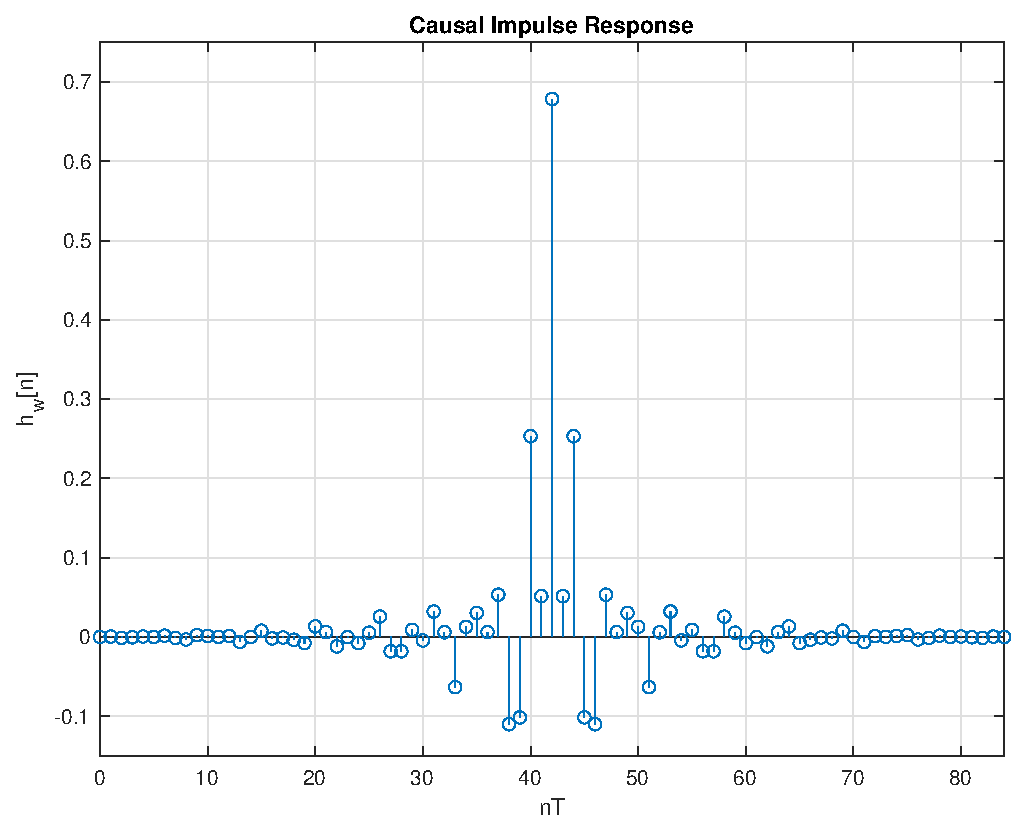
\includegraphics[scale=0.6]{cir.eps} 
    \caption{Causal Impulse Response}
    \label{fig:kaiser}
\end{figure}

\subsection{Magnitude Response of the Digital Filter}
\begin{figure}[H]
    \centering
    \includegraphics[scale=0.6]{mag.eps} 
    \caption{Magnitude Response of the BandStop Filter}
    \label{fig:kaiser}
\end{figure}

\subsection{Magnitude Responses of the Passbands}
\begin{figure}[H]
    \centering
    \begin{minipage}{.5\textwidth}
        \centering
        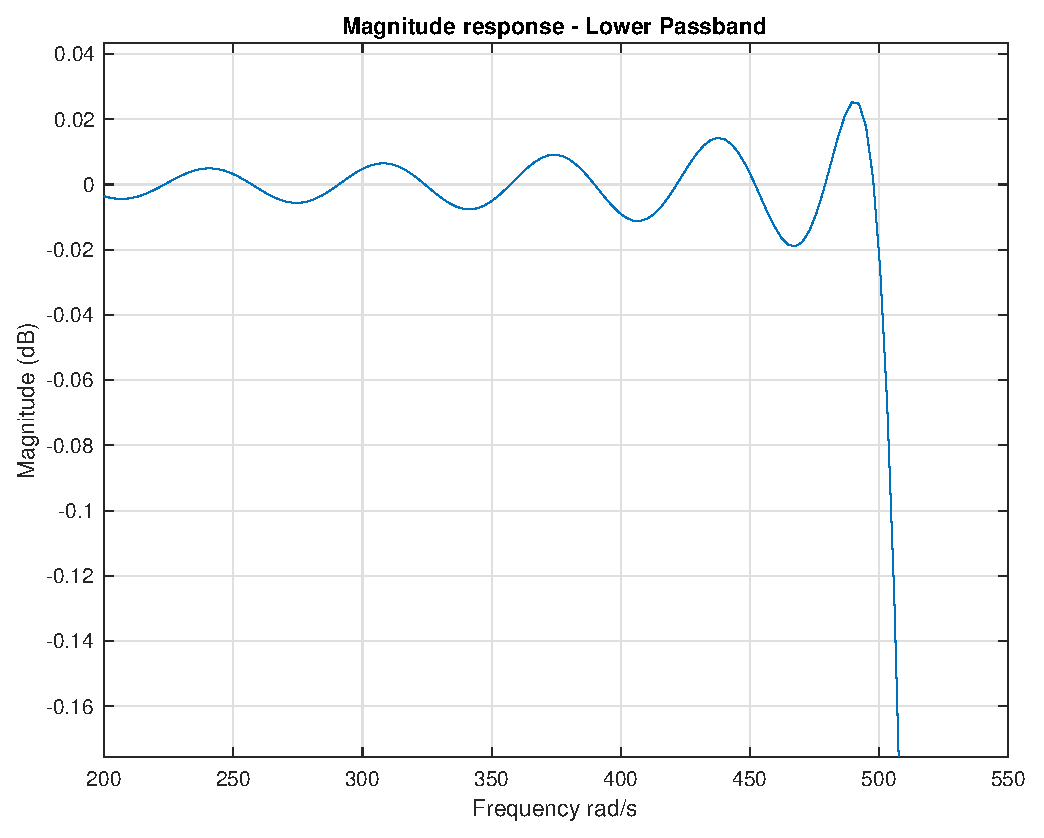
\includegraphics[width=1\linewidth]{upassband.eps}
        \captionof{figure}{Upper passband (Zoomed)}
        \label{fig:test2}
      \end{minipage}%
	\begin{minipage}{.5\textwidth}
	  \centering
	  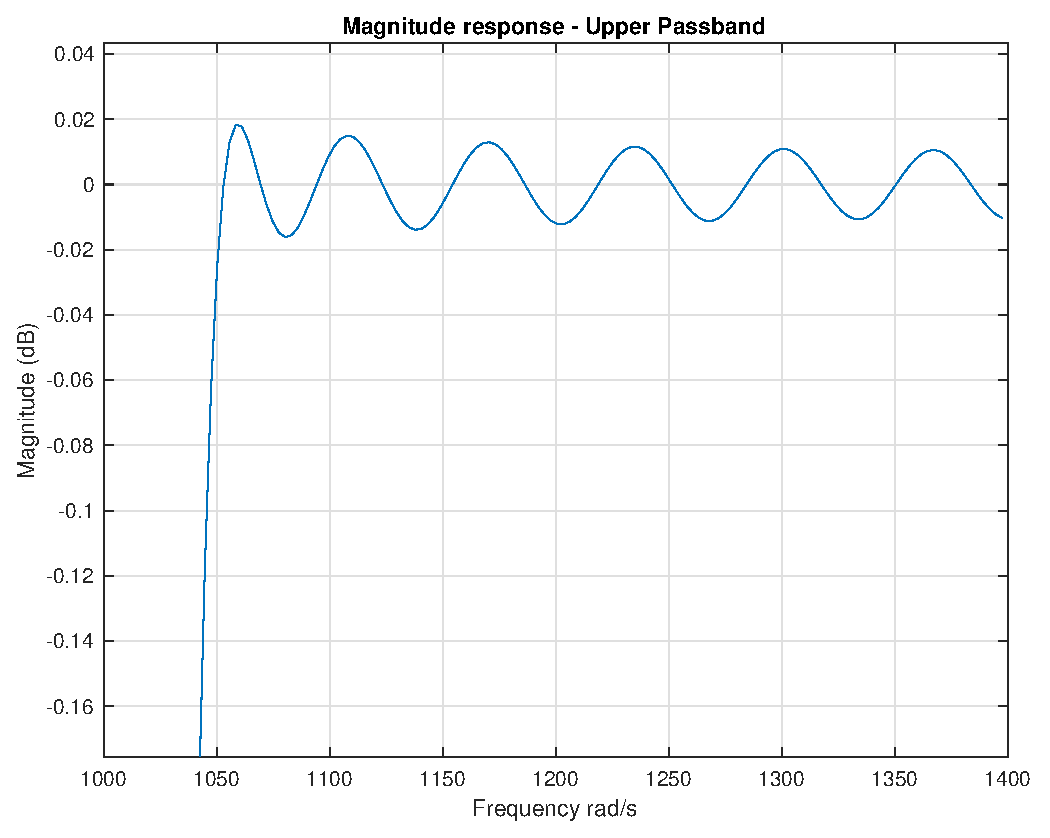
\includegraphics[width=1\linewidth]{lpassband.eps}
	  \captionof{figure}{Lower passband (Zoomed)}
	  \label{fig:test1}
	\end{minipage}
\end{figure}


\subsection{Input Signal}
\begin{figure}[H]
    \centering
    \includegraphics[scale=0.56]{input} 
    \caption{$x( nT) \ =\sum ^{3}_{i=1} cos[ \Omega _{i} nT]$}
\end{figure}
\begin{figure}[H]
    \centering
    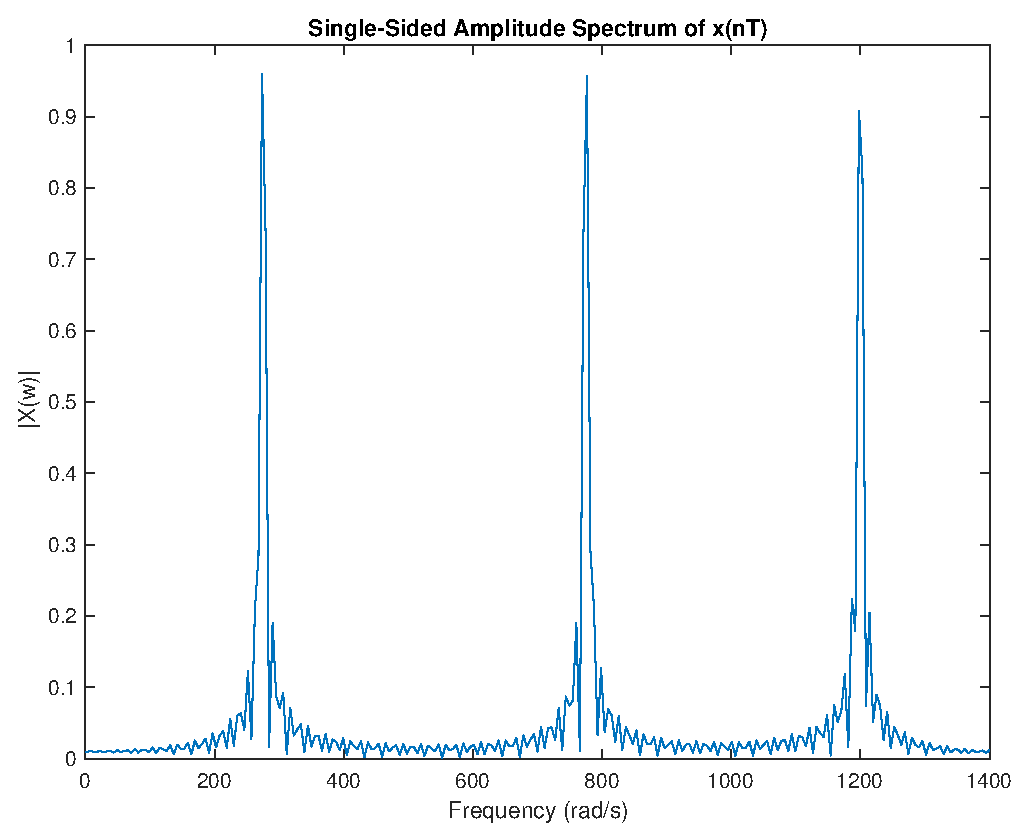
\includegraphics[scale=0.45]{Xw.eps} 
\end{figure}

\subsection{Filtered Signal}
$$Input\ Signal: \ \ x( nT) \ =\sum ^{3}_{i=1} cos[ \Omega _{i} nT]$$
\begin{figure}[H]
    \centering
    \includegraphics[scale=0.6]{filtered} 
    \caption{$x( nT) \ *\ h_{w}( nT)$}
\end{figure}

\begin{figure}[H]
    \centering
    \includegraphics[scale=0.6]{filtered_mag} 
    \caption{$\mathscr{F} \ ( x( nT) \ *\ h_{w}( nT))$}
\end{figure}

\subsection{Expected Outputs}

\begin{figure}[H]
    \centering
    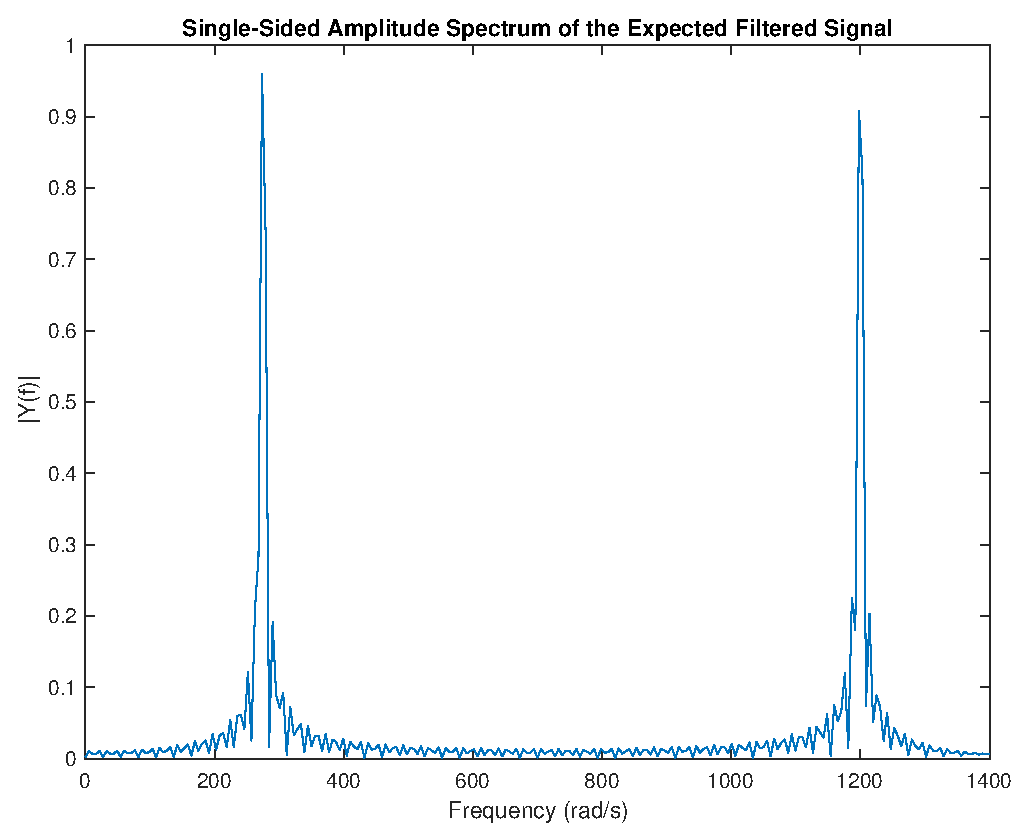
\includegraphics[scale=0.6]{efs.eps} 
    \caption{$\mathscr{F} \ ( cos[ \Omega _{1} nT] \ +\ cos[ \Omega _{3} nT])$}
\end{figure}

\newpage
\bibliographystyle{unsrt}
\bibliography{References}


\end{document}

